\chapter{Results}
\label{chap:results}

All experiments conducted are about assembling target polyominoes with the use of our global planner (\autoref{chap:global}).
In \autoref{sec:AFN} we analyze the effect of increasing target sizes on planning time, rotational cost and other global planner characteristics mentioned in \autoref{sec:global_complex}.
The polyominoes of this experiment are randomly generated, but we also evaluate the construction of manually designed polyominoes in \autoref{sec:AFTS}.
With these polyominoes, we can specifically test the assembly of targets with caves or holes, varying widths and heights, or different patterns of red and blue cubes. 
Furthermore, we experiment with different workspace sizes and aspect ratios in \autoref{sec:AFBS}.
We run all these experiments with the three option sorting strategies of \autoref{sec:connect_options},
\begin{enumerate}
	\item Minimal Distance (MIN DIST)
	\item Grow Largest Component (GROW LARGEST)
	\item Grow Smallest Component (GROW SMALLEST)
\end{enumerate}

The experiments were done on multiple computers with the same hardware specification (\textbf{AMD Ryzen 7 5800X @ 8x3.8GHz (-4.7 GHz), 128GB RAM}) running Ubuntu 22.04.2 LTS.

For the creation of random polyominoes and initial configurations we used a seed-based pseudorandom number generator to make the experiments reproducible.
That way the option sorting strategies are applied to the same set of seeds to make the results comparable.
The global planner states a timeout failure after a planning time of $600$ seconds.


\section{Assembly for Target Size}
\label{sec:AFN}

This experiment was conducted with randomly generated initial configuration and randomly generated polyominoes of specific target sizes $n$.
To maximize the variety of possible polyomino-shapes the number of red cubes is set to $n_\textit{red} = \lfloor \frac{n}{2} \rfloor$ \cite{Lu2021}.
Because of the variety, this experiment is well-suited for not only analyzing planning time and rotational-cost, but also examine $\#\textit{local}$, $\#\textit{config}$ and $|P|$.
We worked in a quadratic workspace of size $50 r_C \times 50 r_C$ and for each target size $150$ samples were taken.

\paragraph{Time and Failure Analysis}

\begin{figure}
	\centering
	\begin{subfigure}[b]{\textwidth}
		\centering
		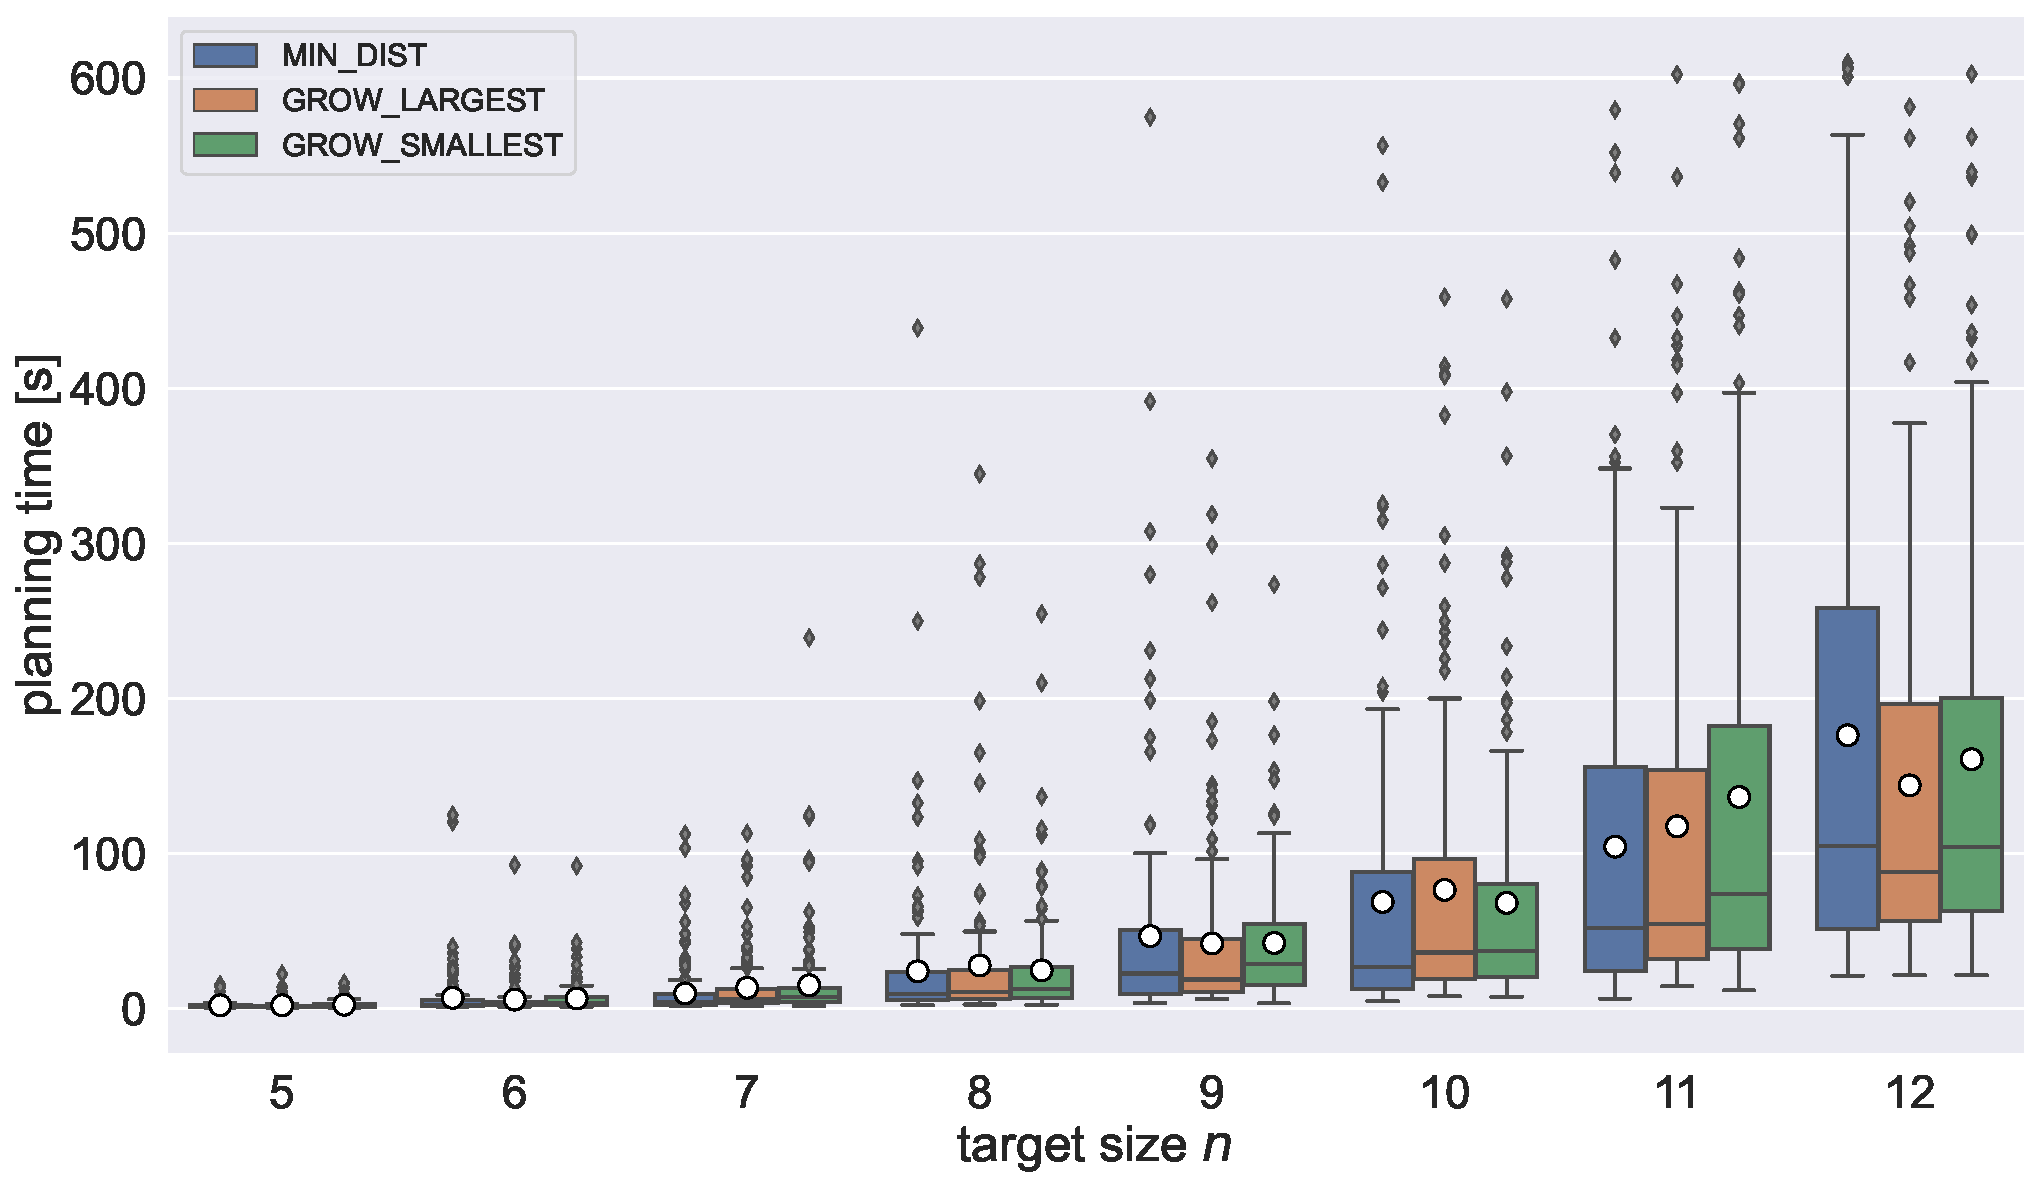
\includegraphics[width=0.9\textwidth]{figures/plots/AFN_time.pdf}
		\caption{Planning time in seconds. Only plans that did not time out are shown.}
		\label{fig:AFN_time}
	\end{subfigure}

	\begin{subfigure}[b]{\textwidth}
		\centering
		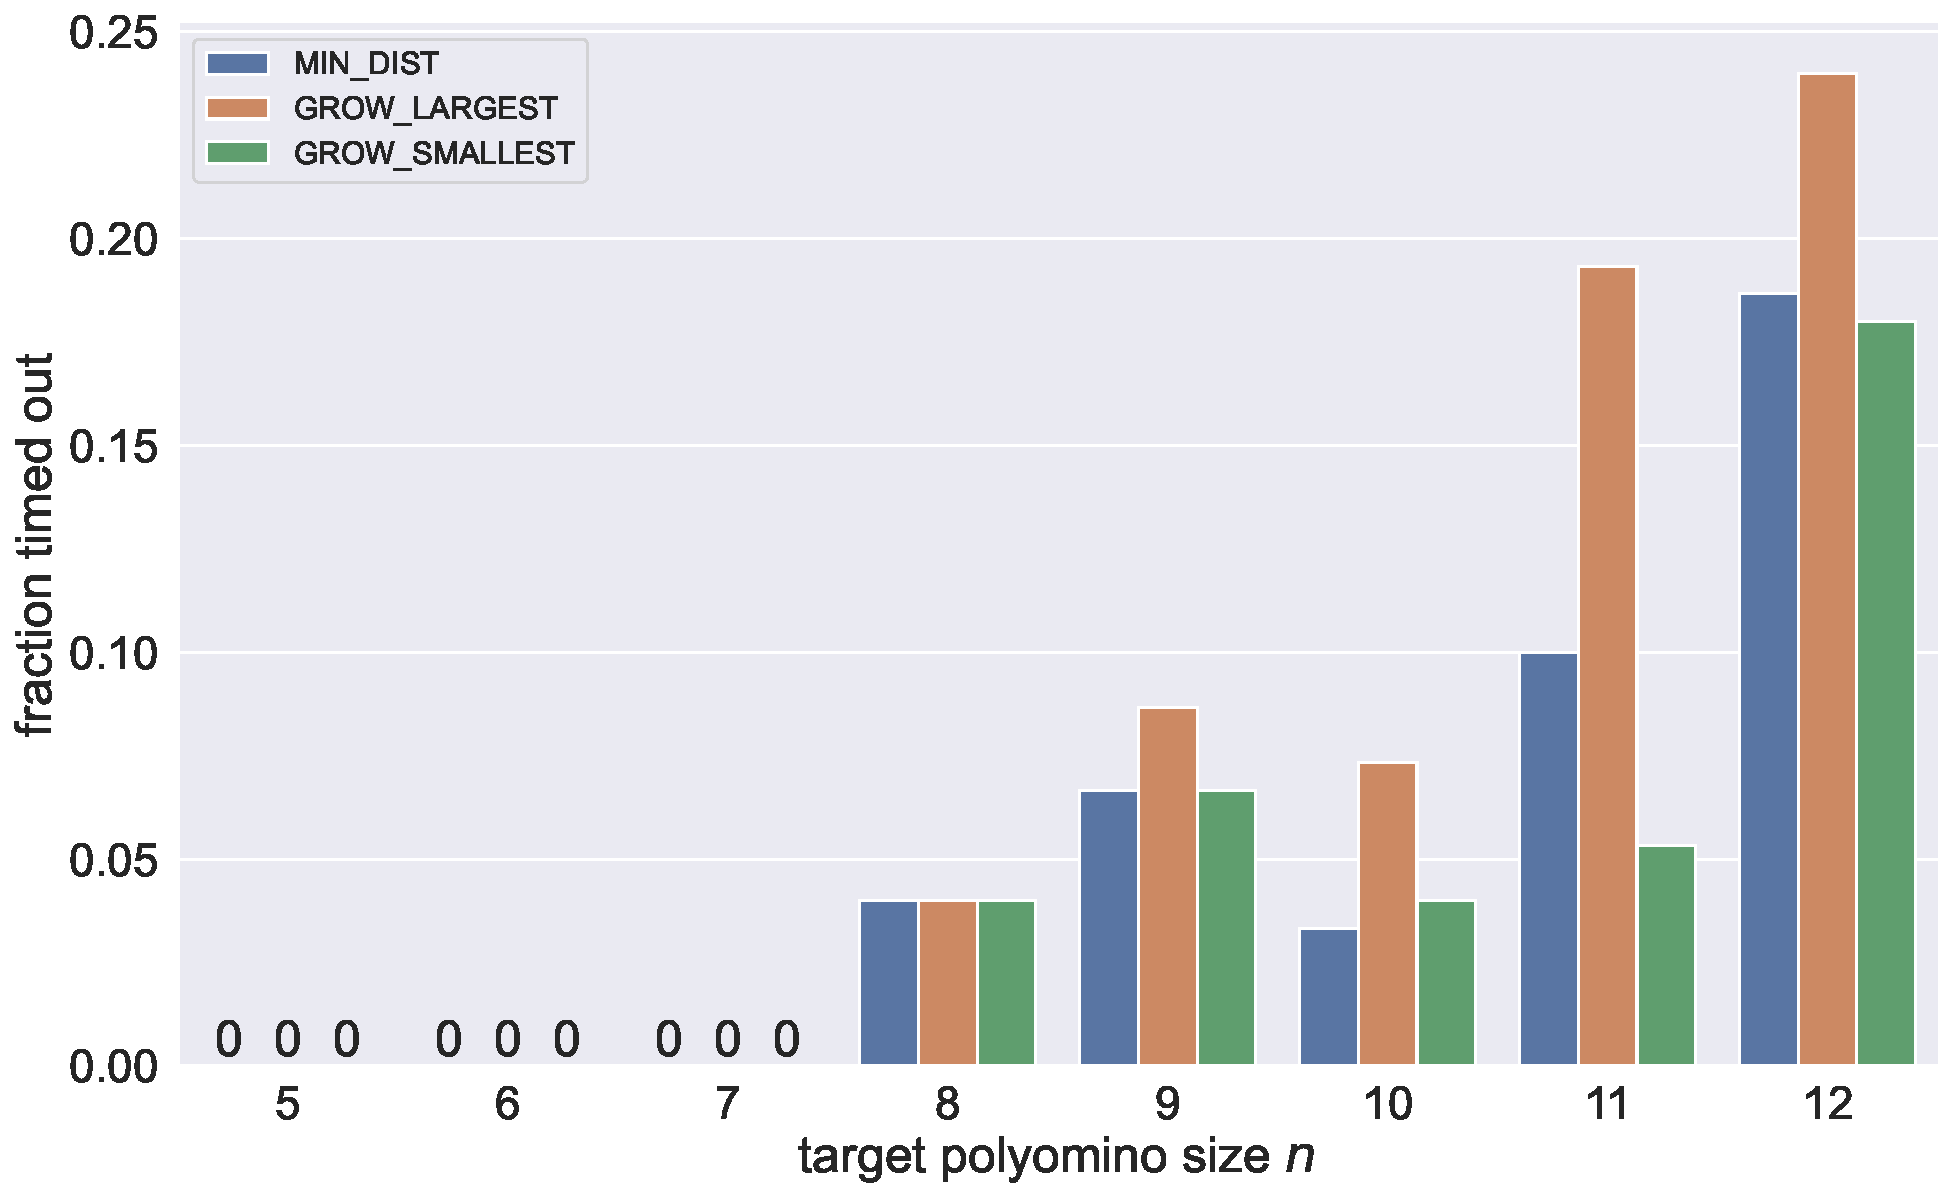
\includegraphics[width=0.9\textwidth]{figures/plots/AFN_timeout.pdf}
		\caption{Fraction of plans that timed out}
		\label{fig:AFN_timeout}
	\end{subfigure}
	\caption[Planning time and fraction timed out for different target sizes]{Planning time and fraction timed out for different target sizes $n$. All option sorting strategies are compared.}
	\label{fig:AFN_timestats}
\end{figure}



\paragraph{Cost Analysis}

\begin{figure}
	\centering
	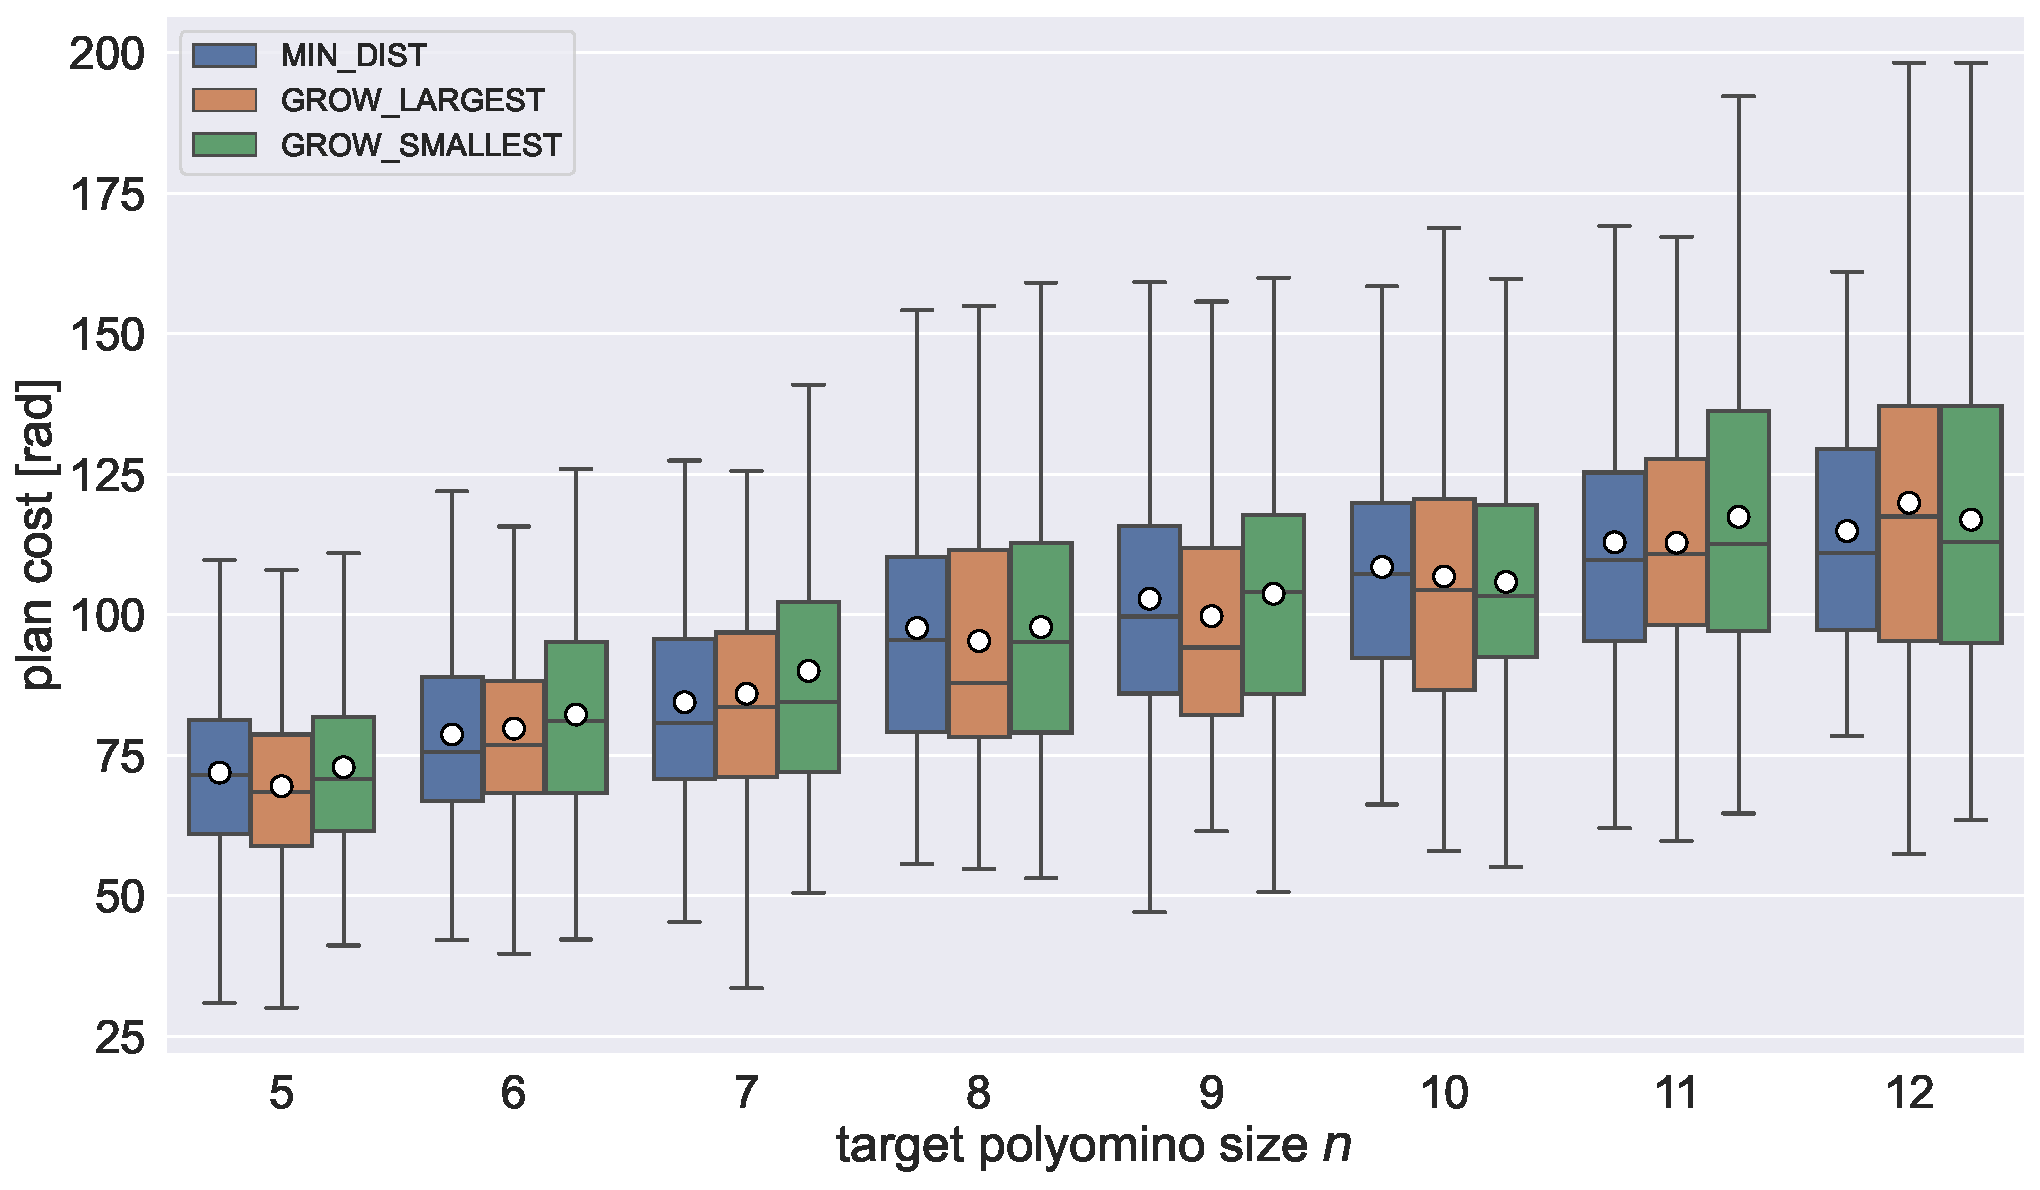
\includegraphics[width=0.9\textwidth]{figures/plots/AFN_cost.pdf}
	\caption[Plan cost for different target sizes]{Plan cost of successful plans for different target sizes $n$. All option sorting strategies are compared.}
	\label{fig:AFN_cost}
\end{figure}



\paragraph{Planning Analysis}

\begin{figure}
	\centering
	\begin{subfigure}[b]{\textwidth}
		\centering
		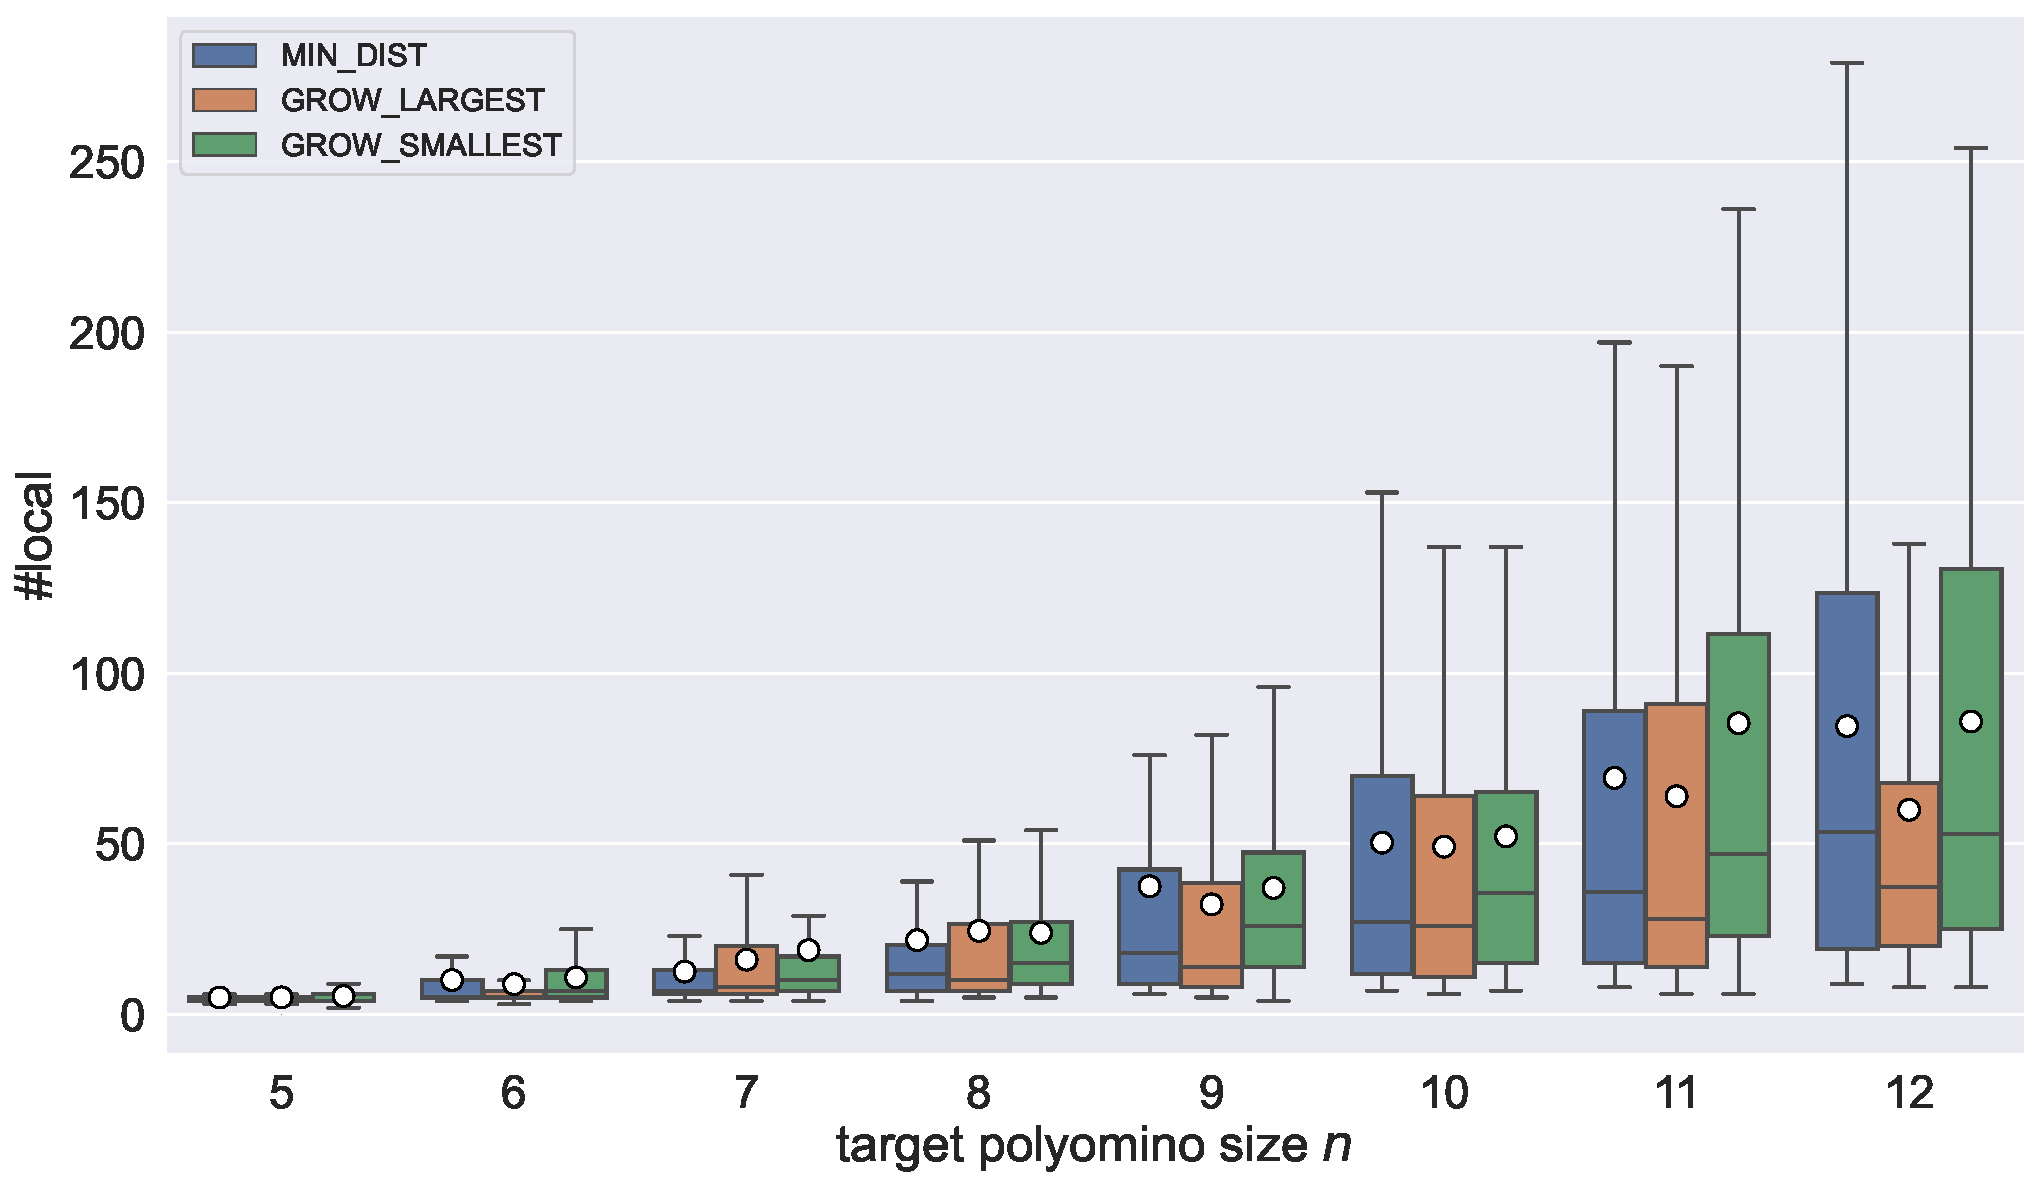
\includegraphics[width=0.9\textwidth]{figures/plots/AFN_nlocal.pdf}
		\caption{Number of simulated local plans.}
		\label{fig:AFN_nlocal}
	\end{subfigure}
	
	\begin{subfigure}[b]{\textwidth}
		\centering
		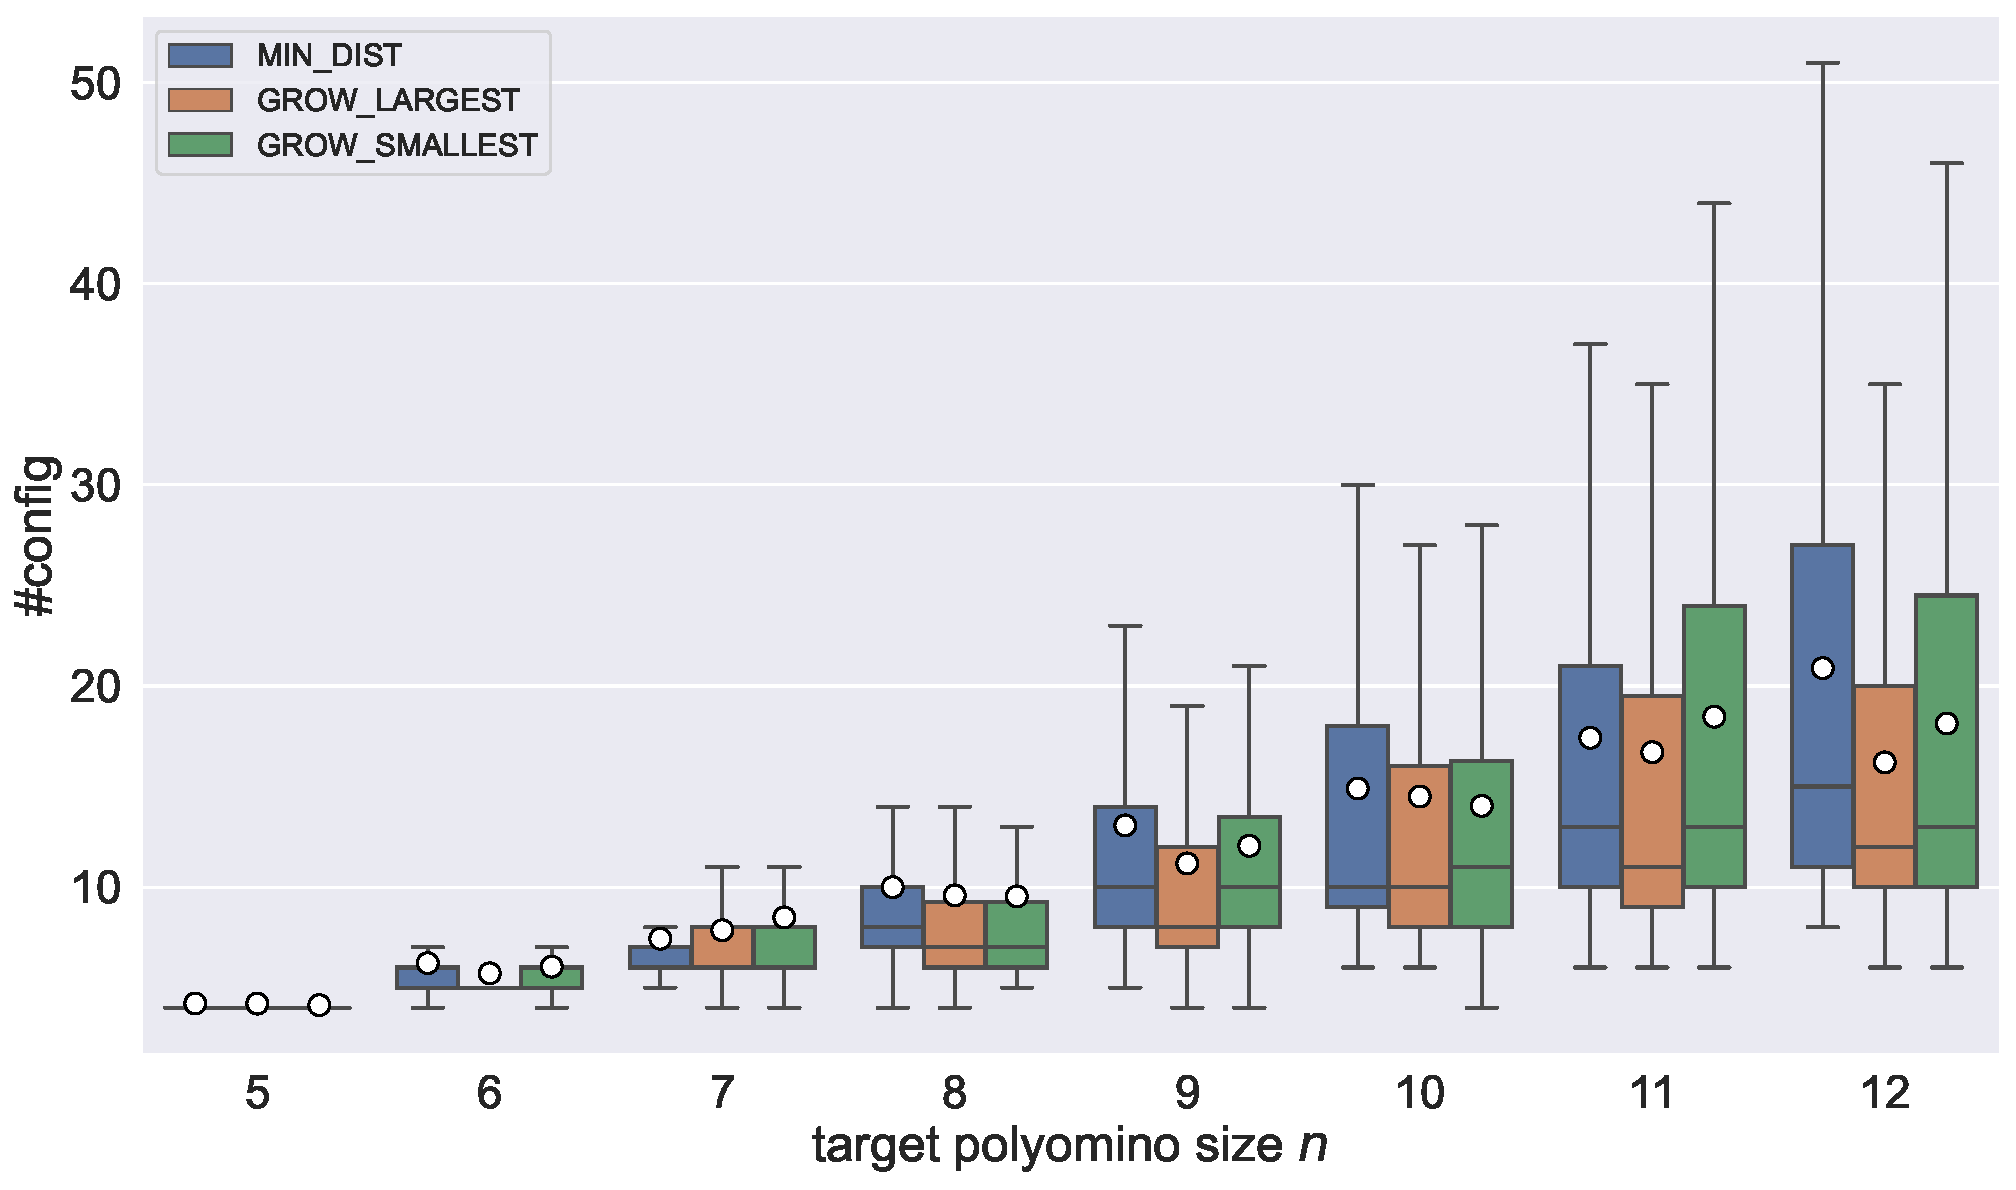
\includegraphics[width=0.9\textwidth]{figures/plots/AFN_nconfig.pdf}
		\caption{Number of explored configurations}
		\label{fig:AFN_nconfig}
	\end{subfigure}
	\caption[$\#\textit{config}$ and $\#\textit{config}$ for different target sizes]{Number of simulated local plans $\#\textit{local}$ and number of explored configurations $\#\textit{config}$ for different target sizes $n$. All option sorting strategies are compared.}
	\label{fig:AFN_planstats}
\end{figure}

\begin{figure}
	\centering
	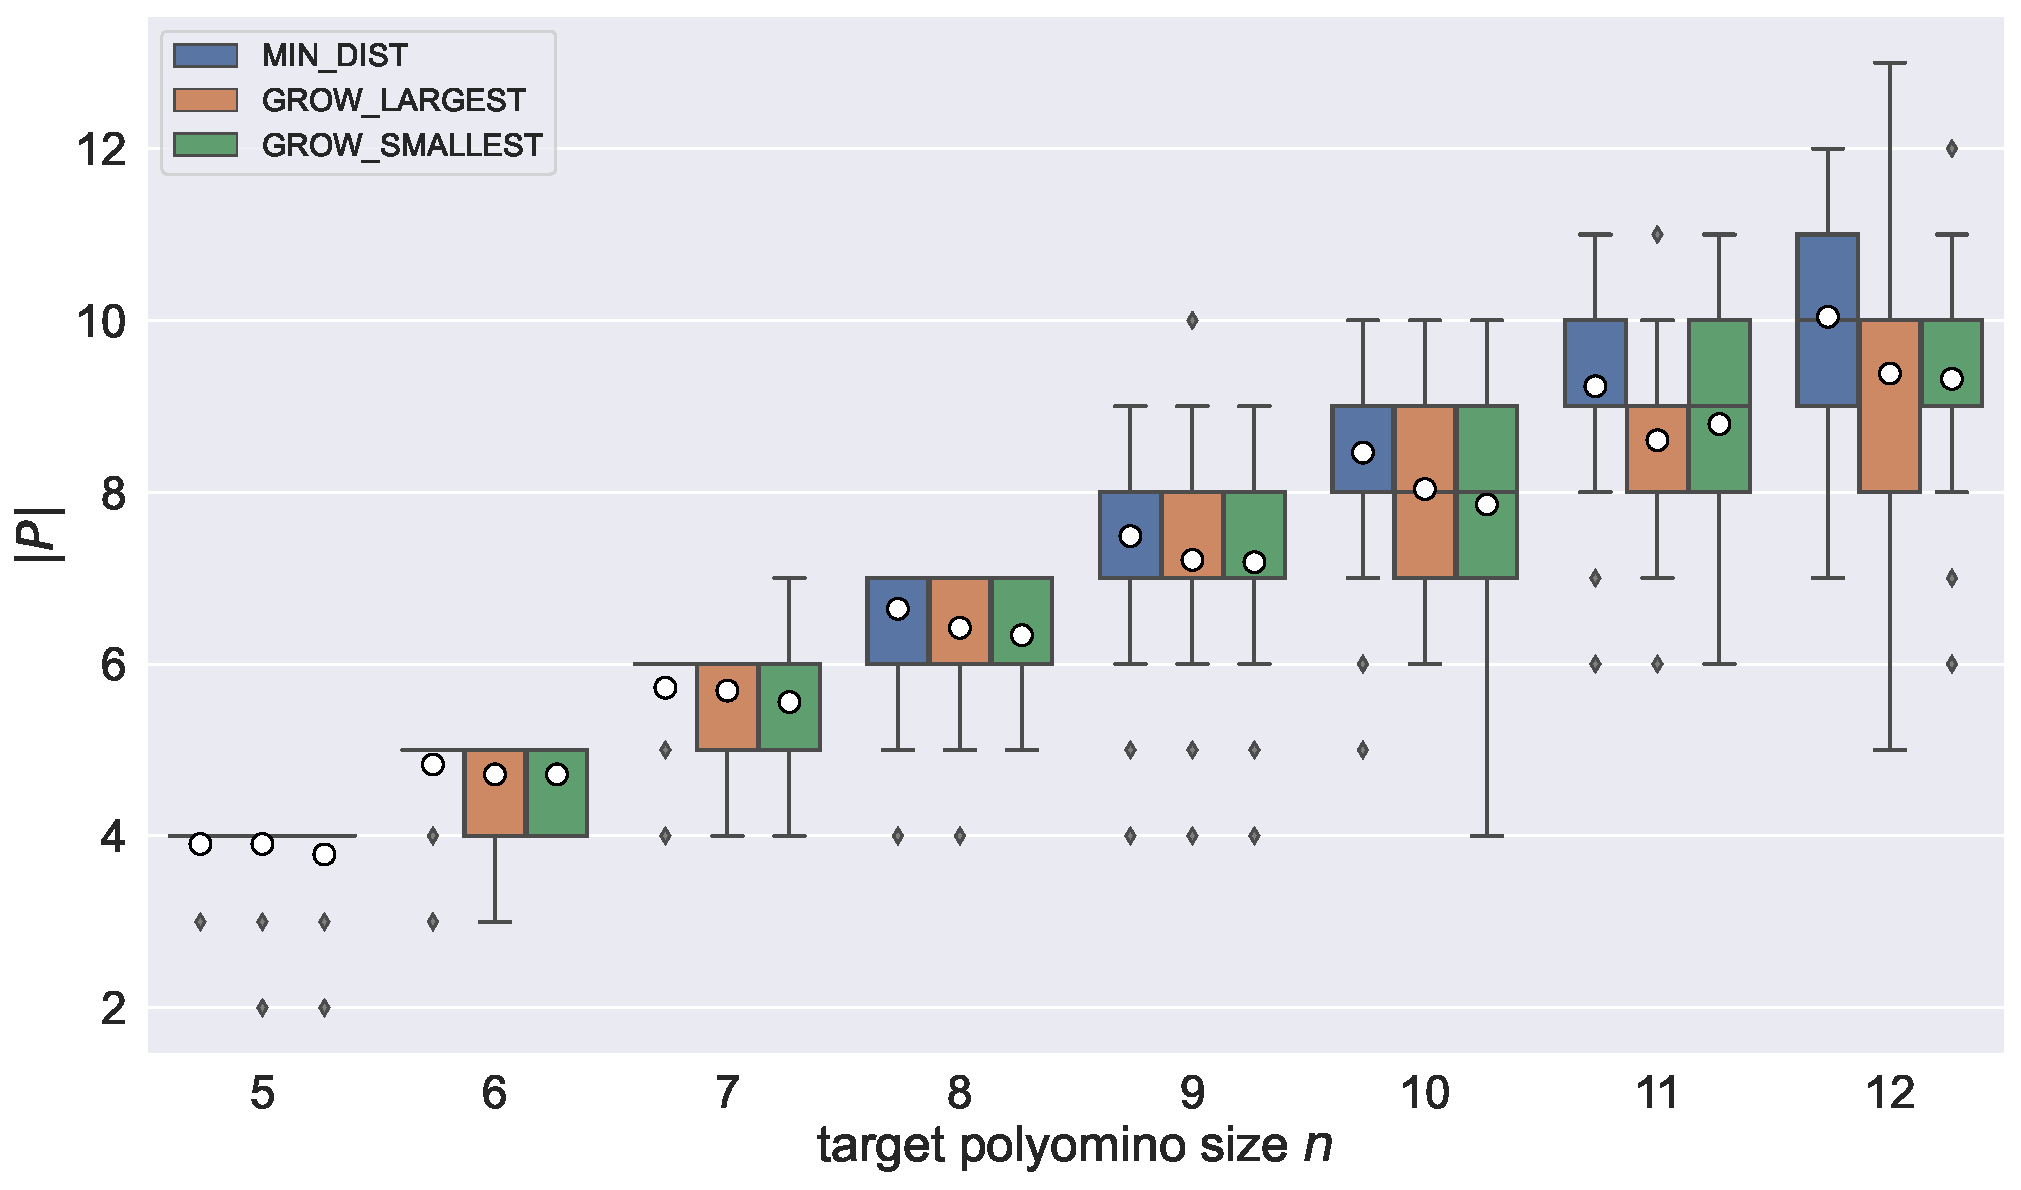
\includegraphics[width=0.9\textwidth]{figures/plots/AFN_ltg.pdf}
	\caption[Local plans in plan stack for different target sizes]{Local plans in plan stack $|P|$ for different target sizes $n$. All option sorting strategies are compared.}
	\label{fig:AFN_ltg}
\end{figure}




\section{Assembly for Target Shape}
\label{sec:AFTS}

\begin{figure}
	\centering
	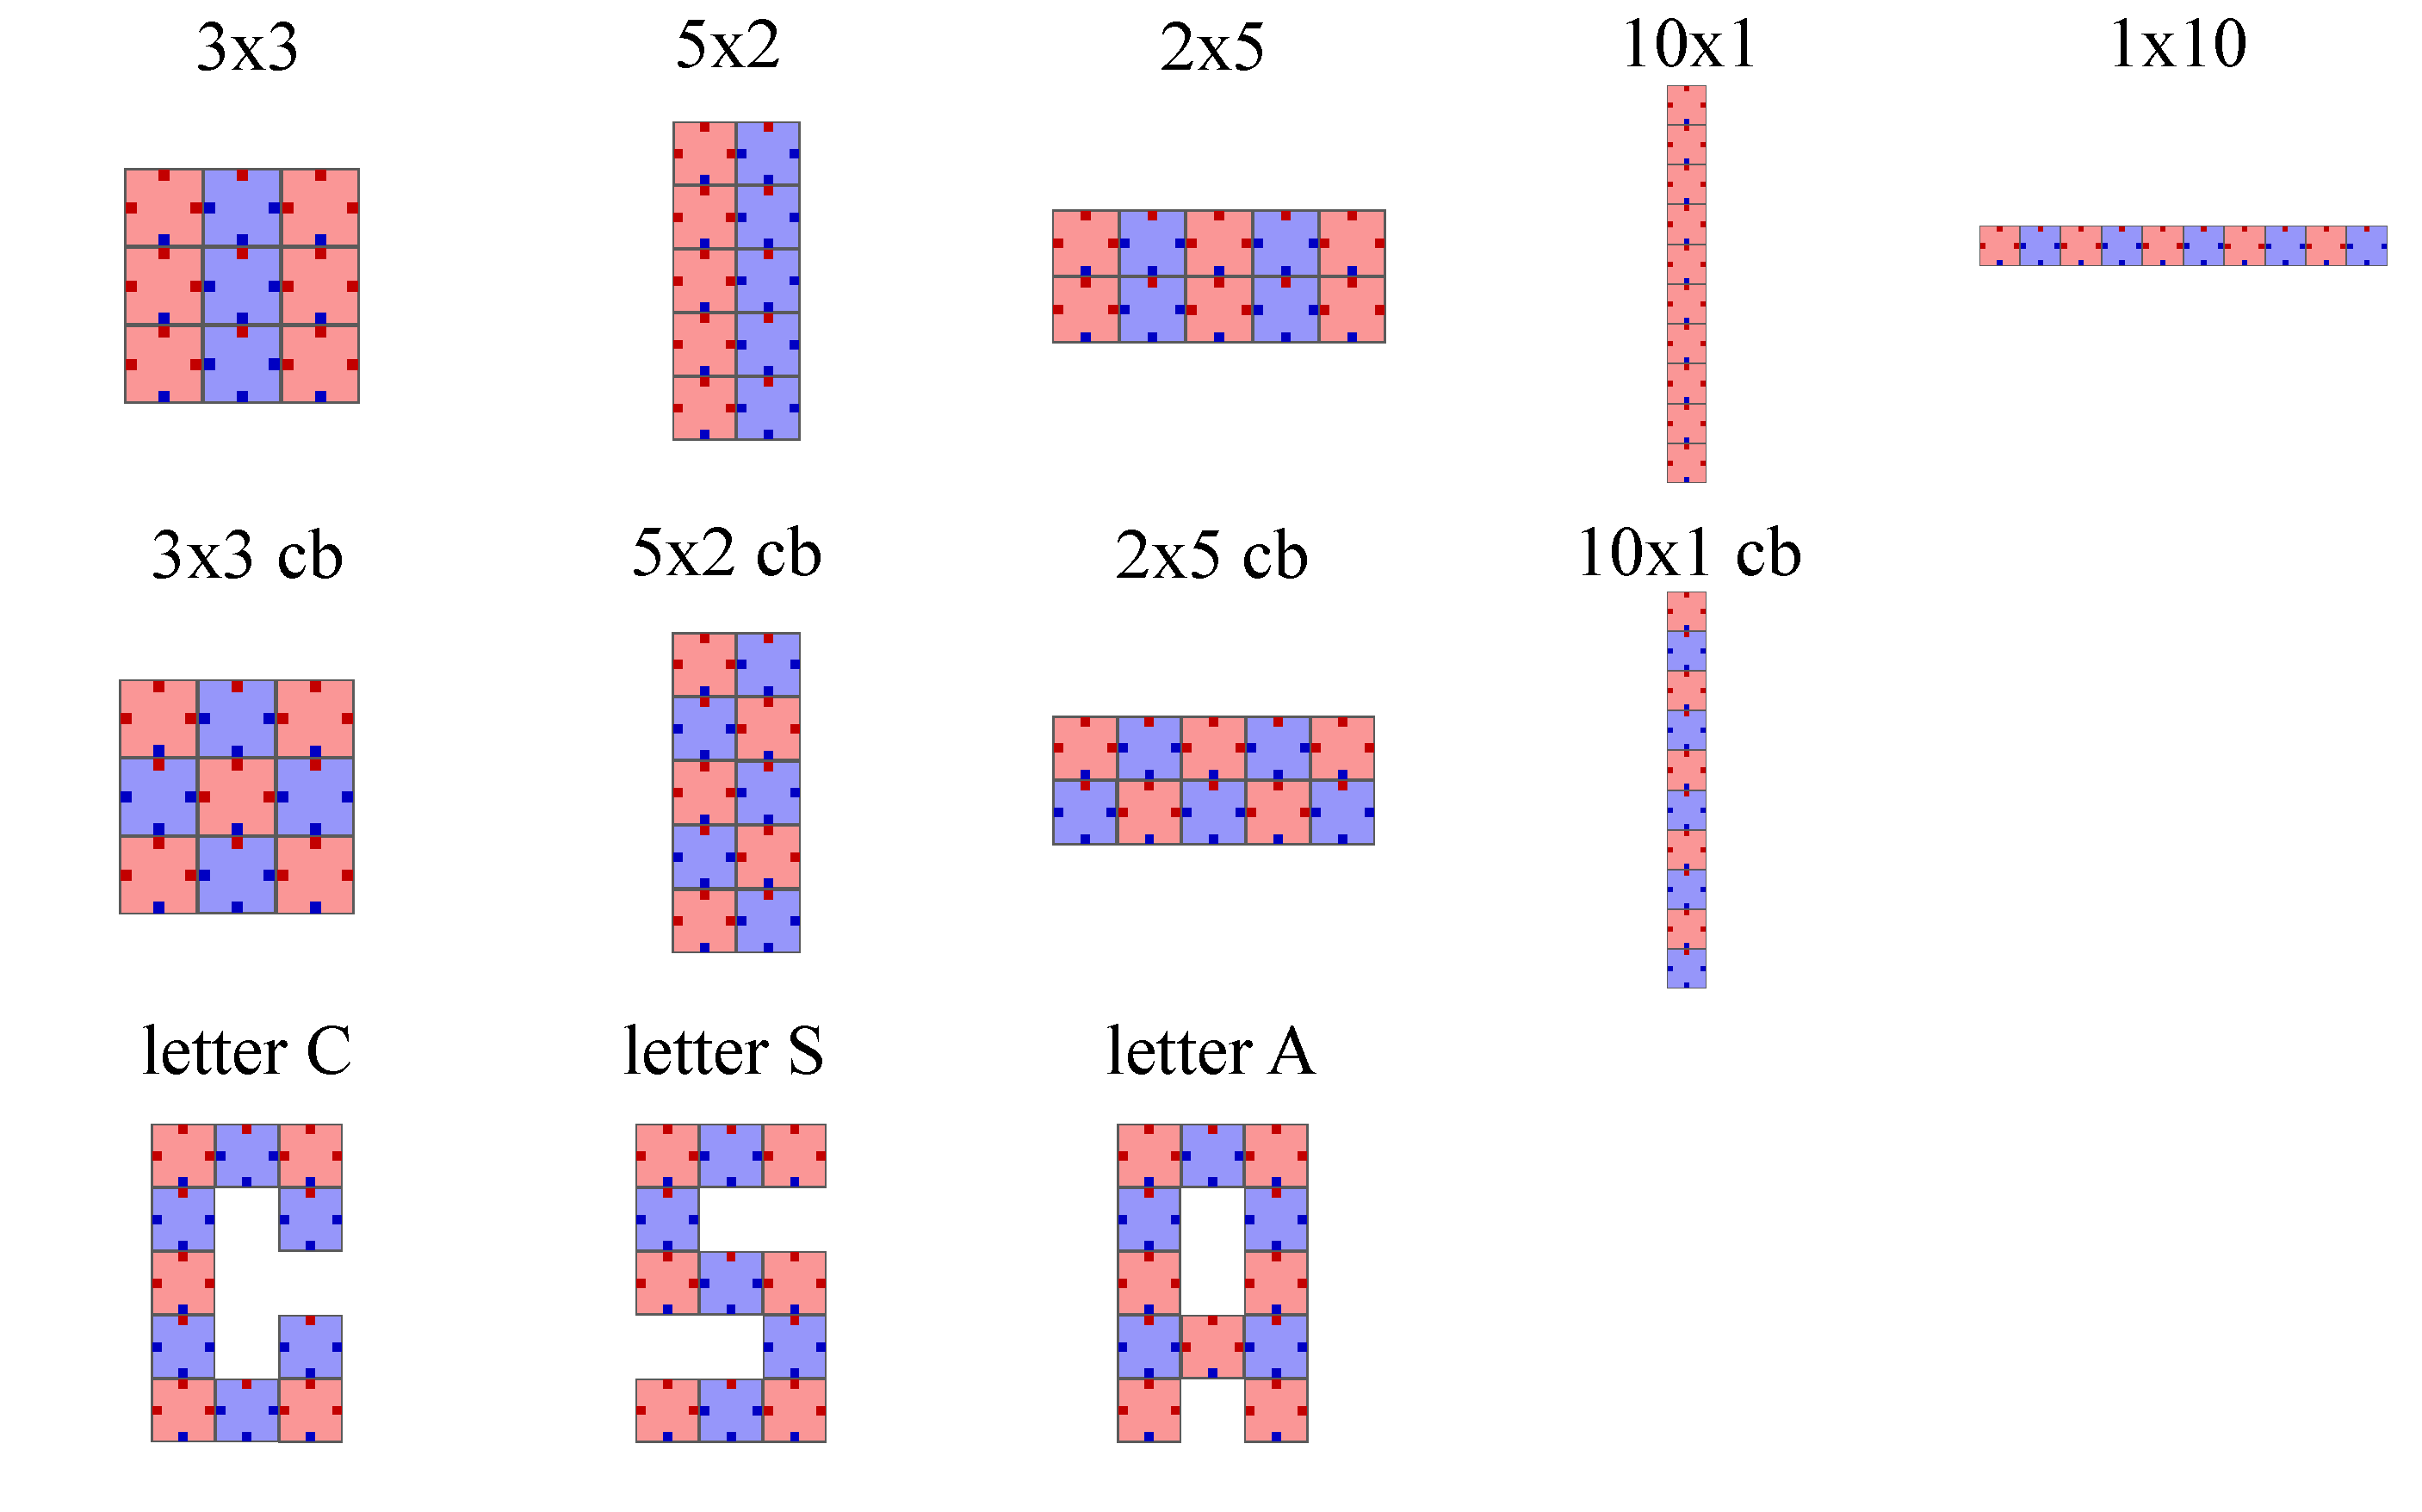
\includegraphics[width=0.8\textwidth]{figures/AFTS_shapes.pdf}
	\caption[List of manually designed polyominoes]{List of manually designed polyominoes for experimenting with special shapes...}
	\label{fig:AFTS_shapes}
\end{figure}


\begin{figure}
	\centering
	\begin{subfigure}[b]{\textwidth}
		\centering
		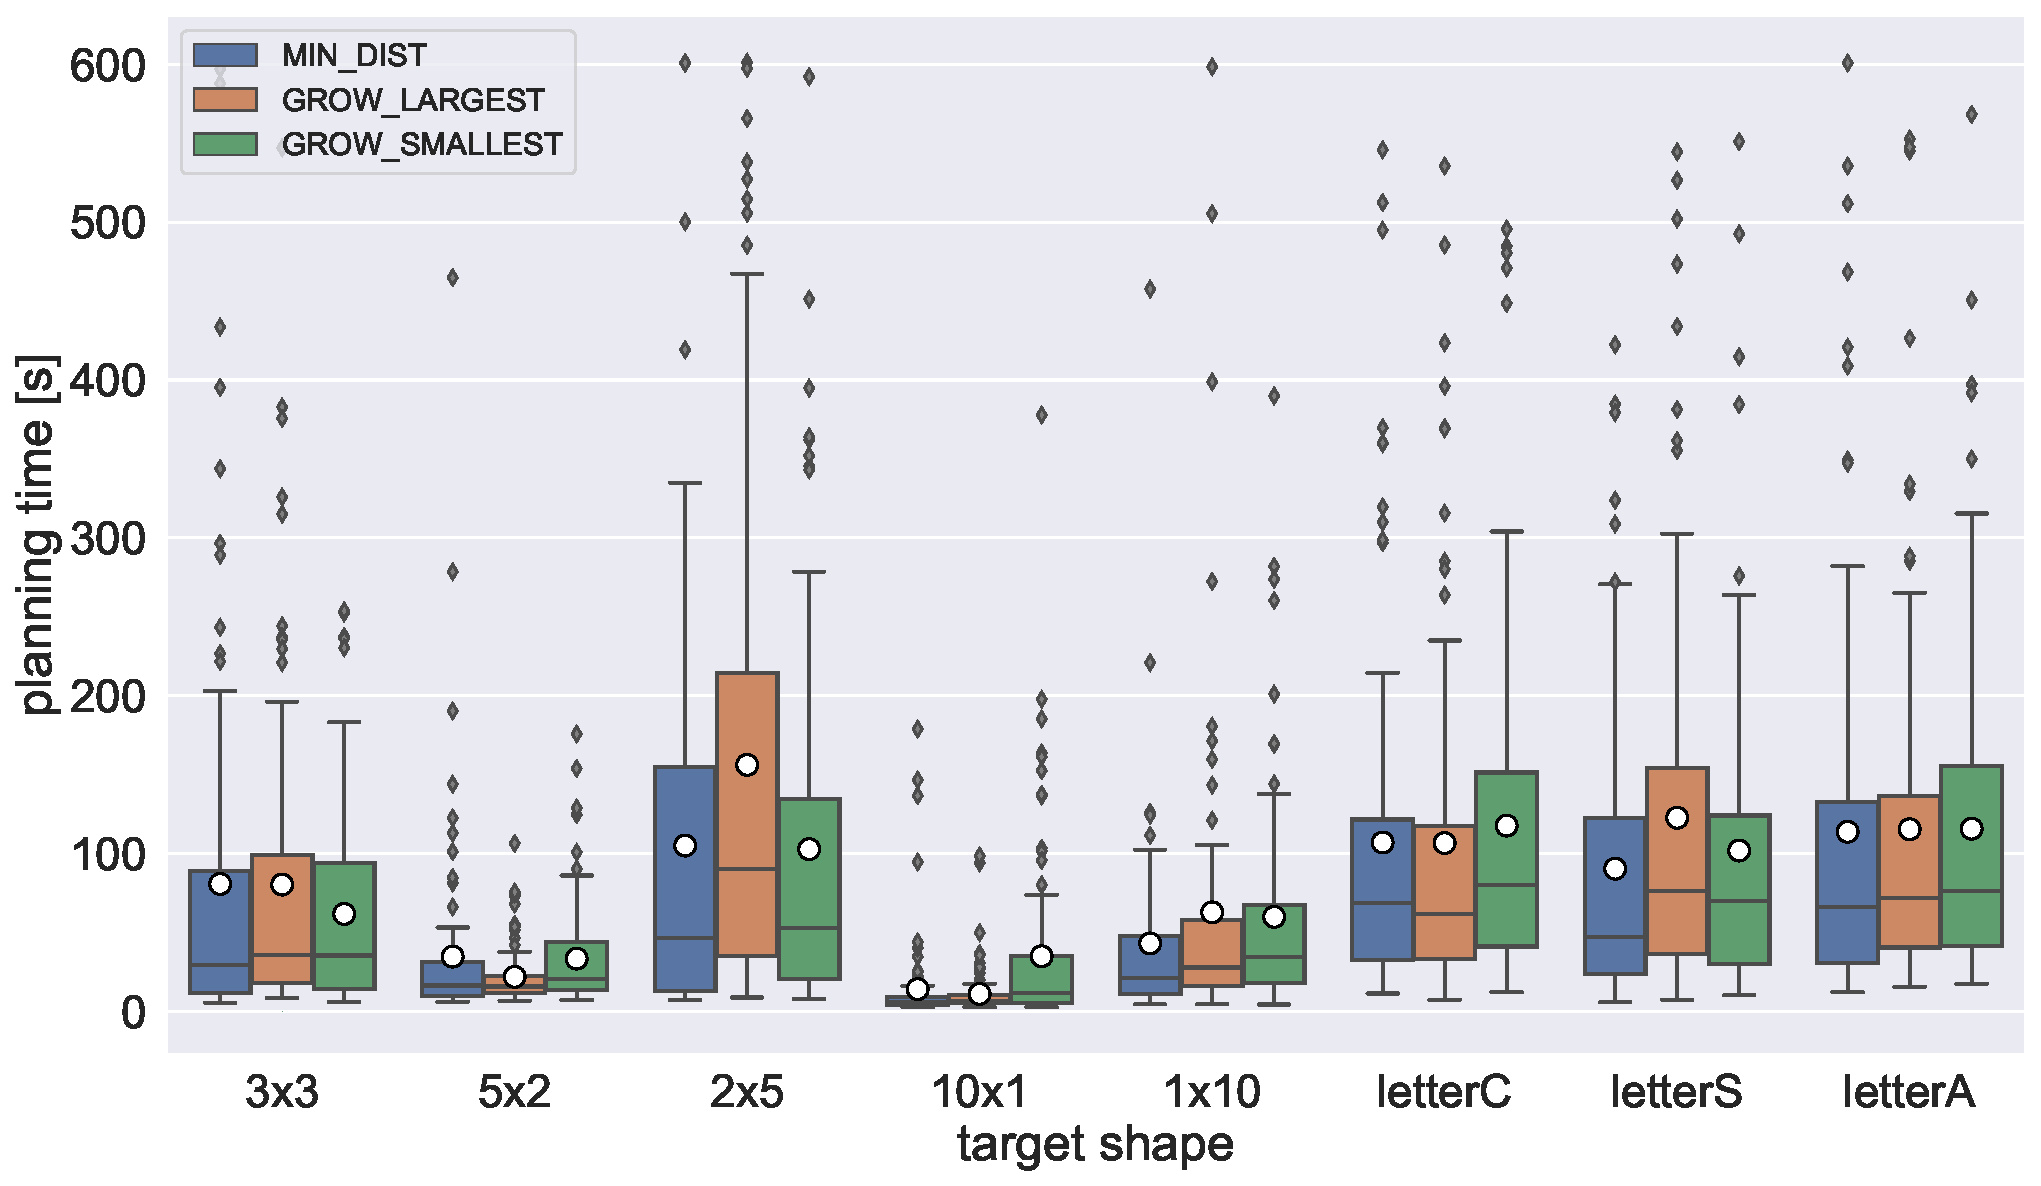
\includegraphics[width=0.9\textwidth]{figures/plots/AFTS_time.pdf}
		\caption{}
		\label{fig:AFTS_time}
	\end{subfigure}
	
	\begin{subfigure}[b]{\textwidth}
		\centering
		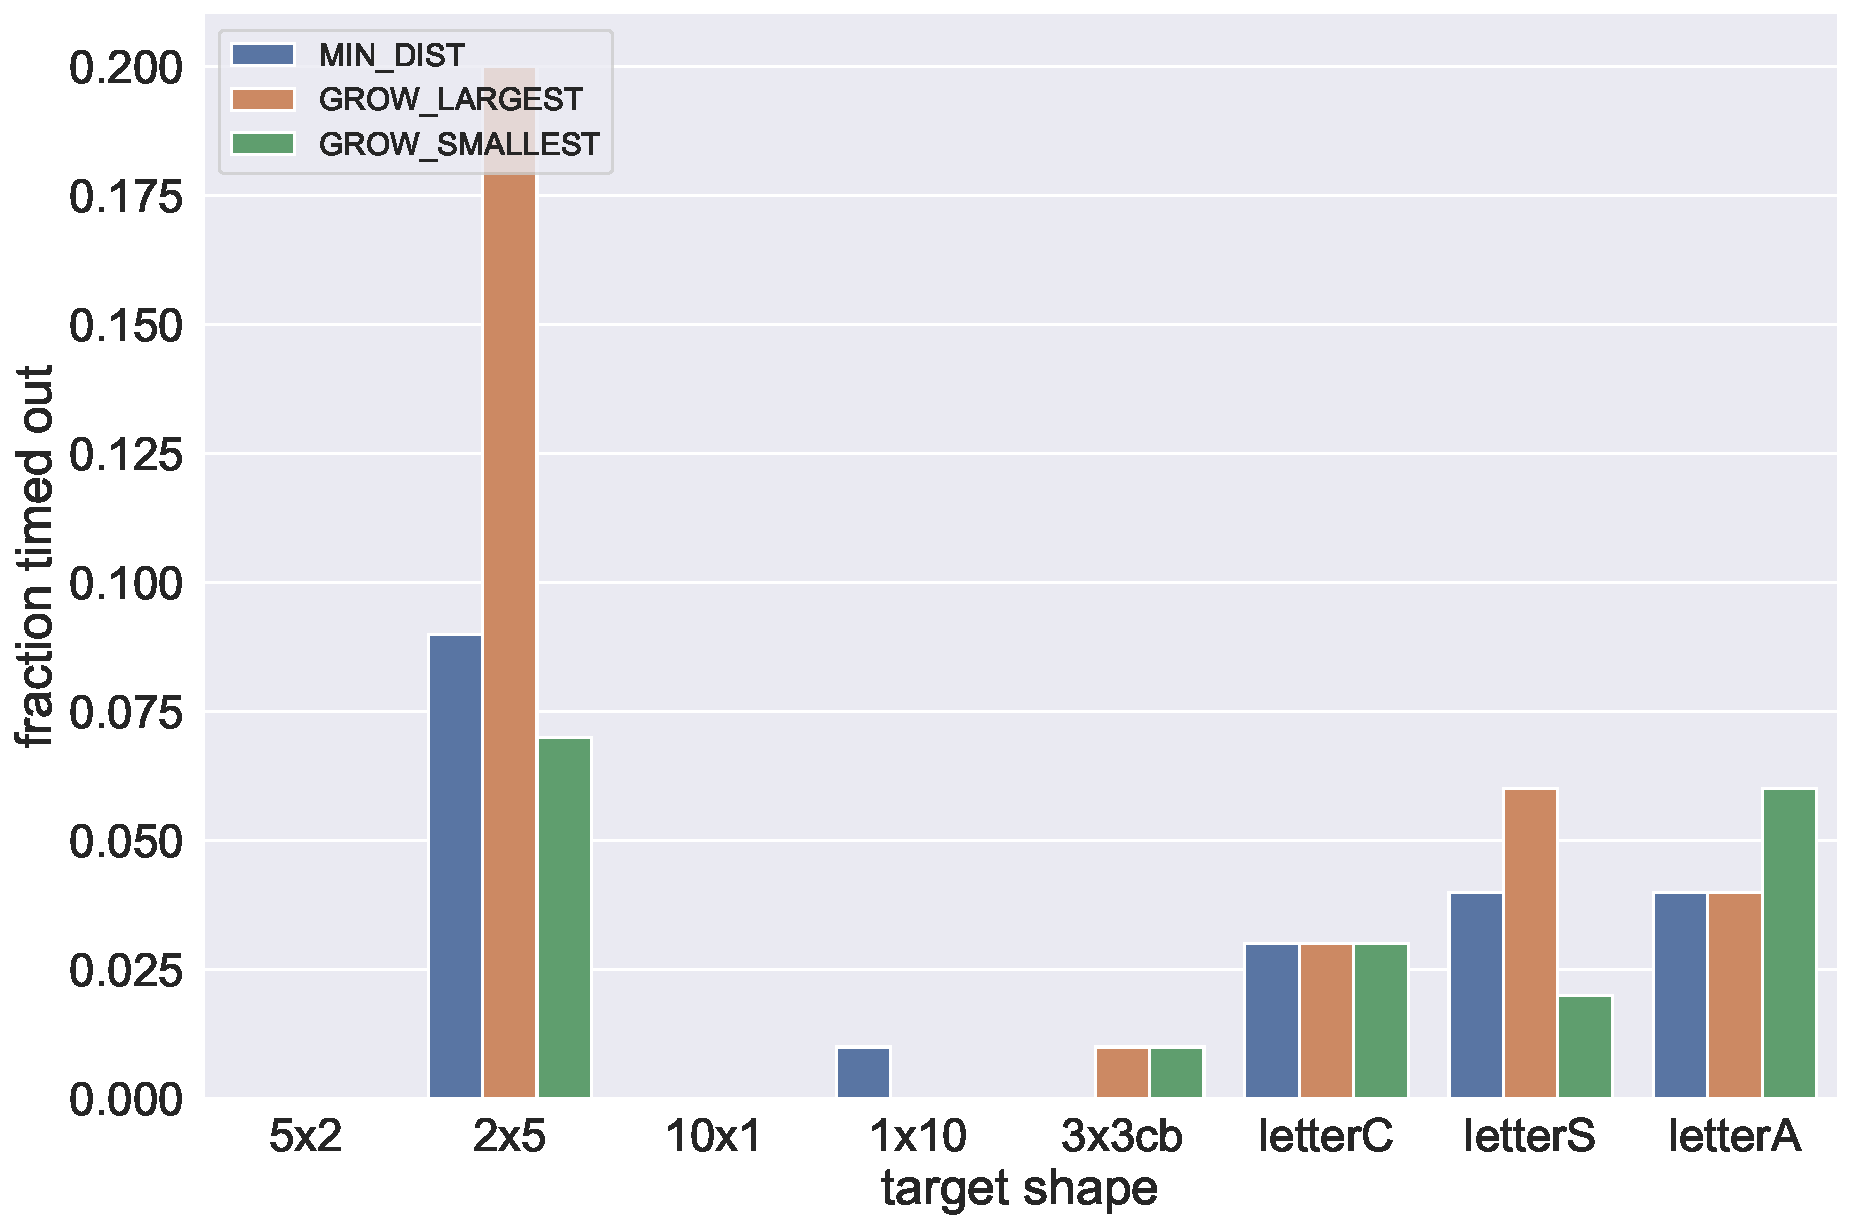
\includegraphics[width=0.9\textwidth]{figures/plots/AFTS_timeout.pdf}
		\caption{}
		\label{fig:AFTS_timeout}
	\end{subfigure}
	\caption[]{}
	\label{fig:AFTS_timestats}
\end{figure}




\section{Assembly for Workspace Size}
\label{sec:AFBS}

\begin{figure}
	\centering
	\begin{subfigure}[b]{\textwidth}
		\centering
		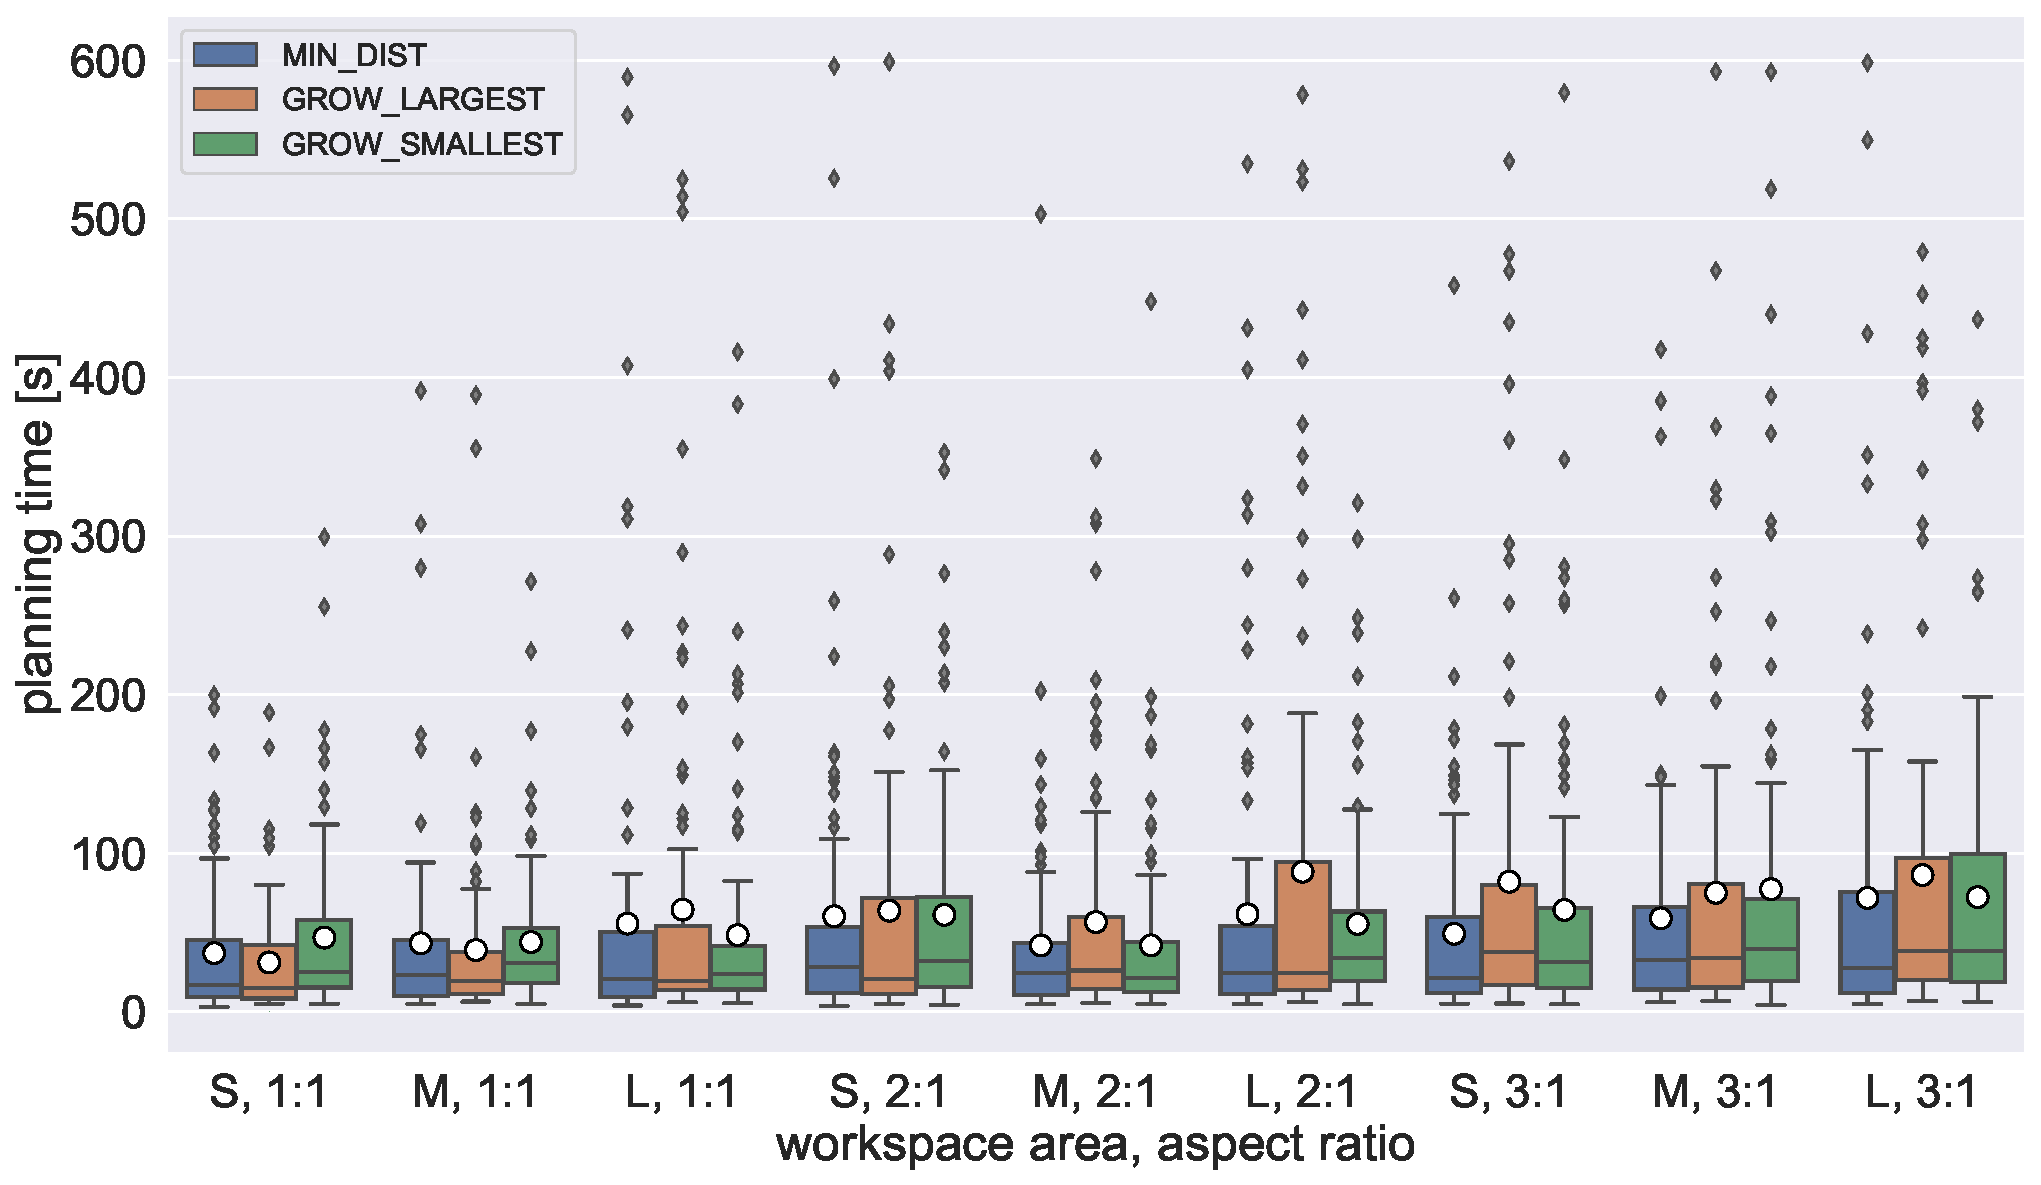
\includegraphics[width=0.9\textwidth]{figures/plots/AFBS_time.pdf}
		\caption{}
		\label{fig:AFBS_time}
	\end{subfigure}
	
	\begin{subfigure}[b]{\textwidth}
		\centering
		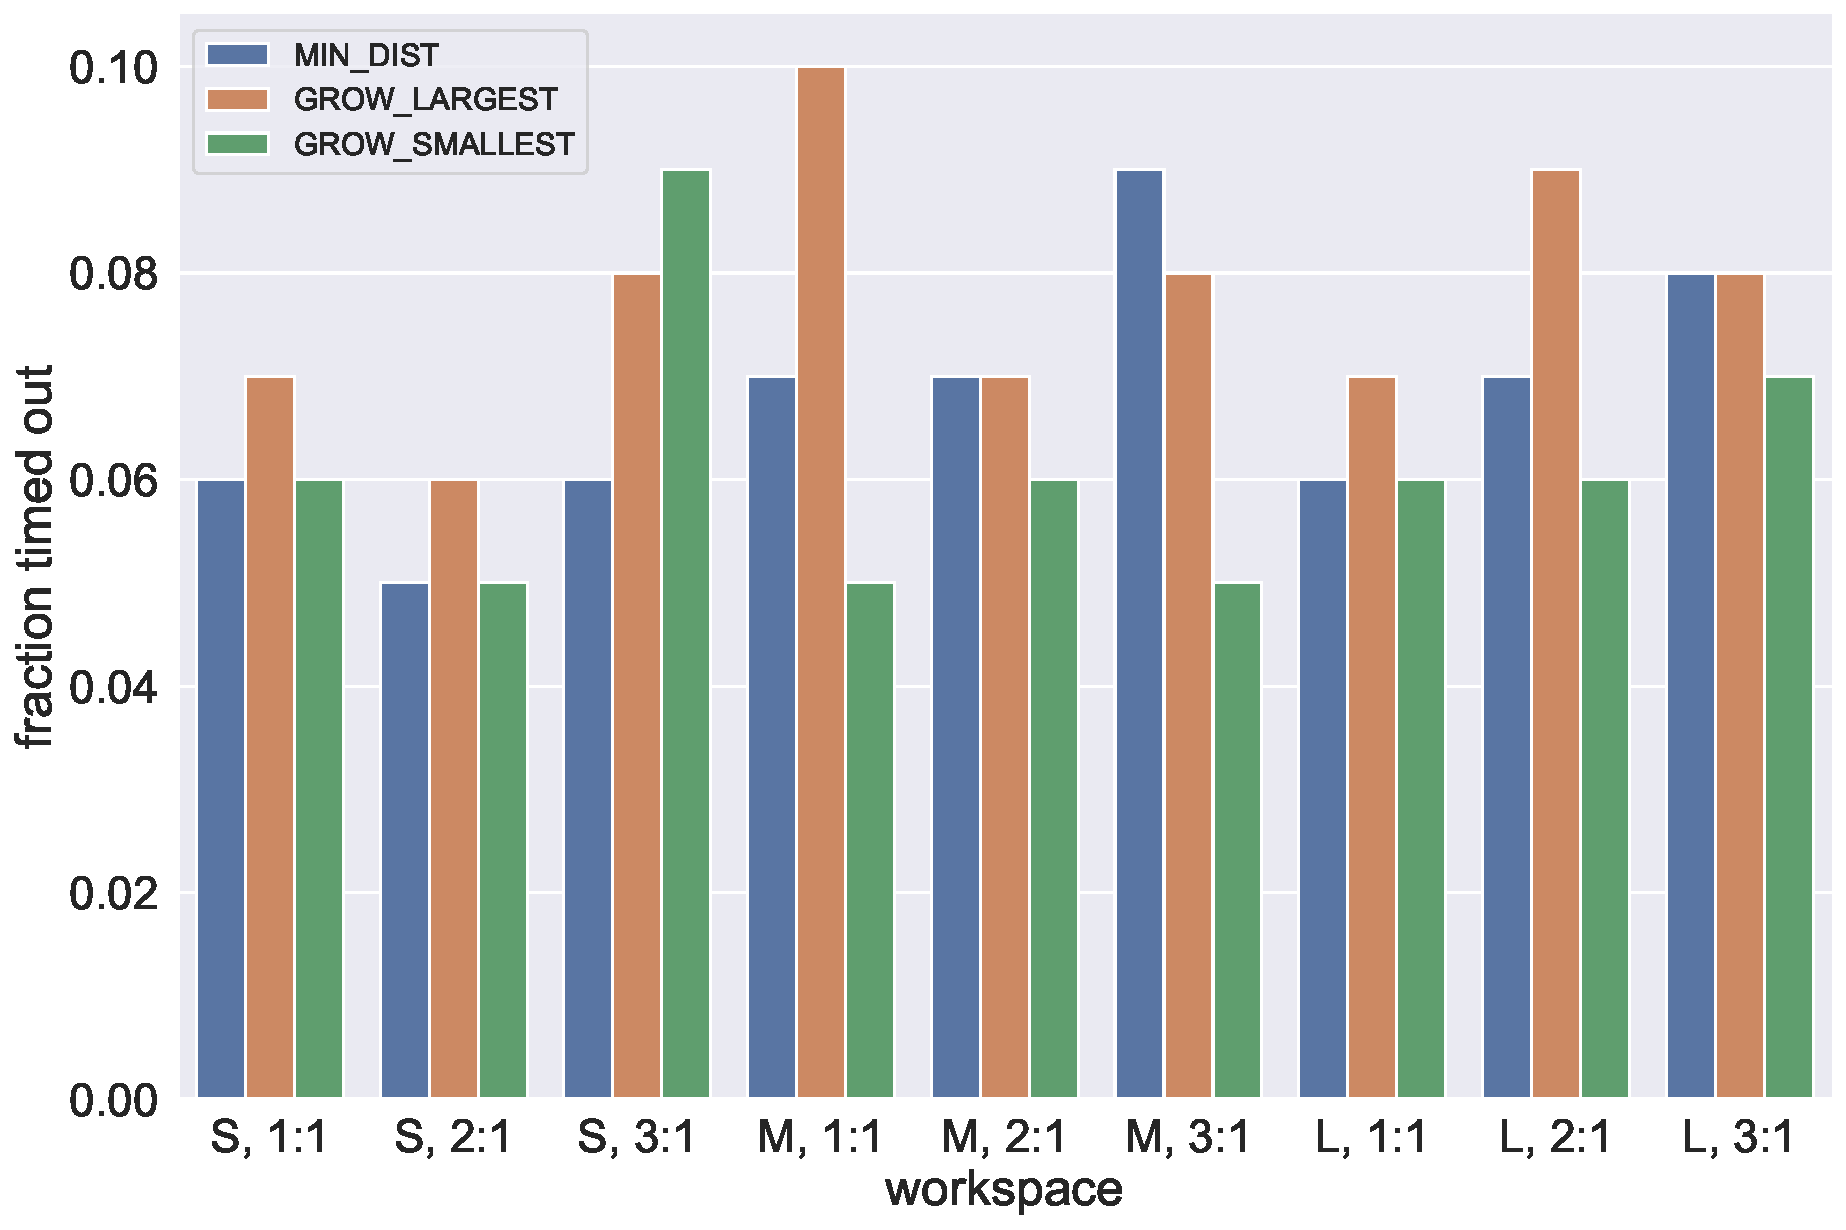
\includegraphics[width=0.9\textwidth]{figures/plots/AFBS_timeout.pdf}
		\caption{}
		\label{fig:AFBS_timeout}
	\end{subfigure}
	\caption[]{}
	\label{fig:AFBS_timestats}
\end{figure}

\begin{figure}
	\centering
	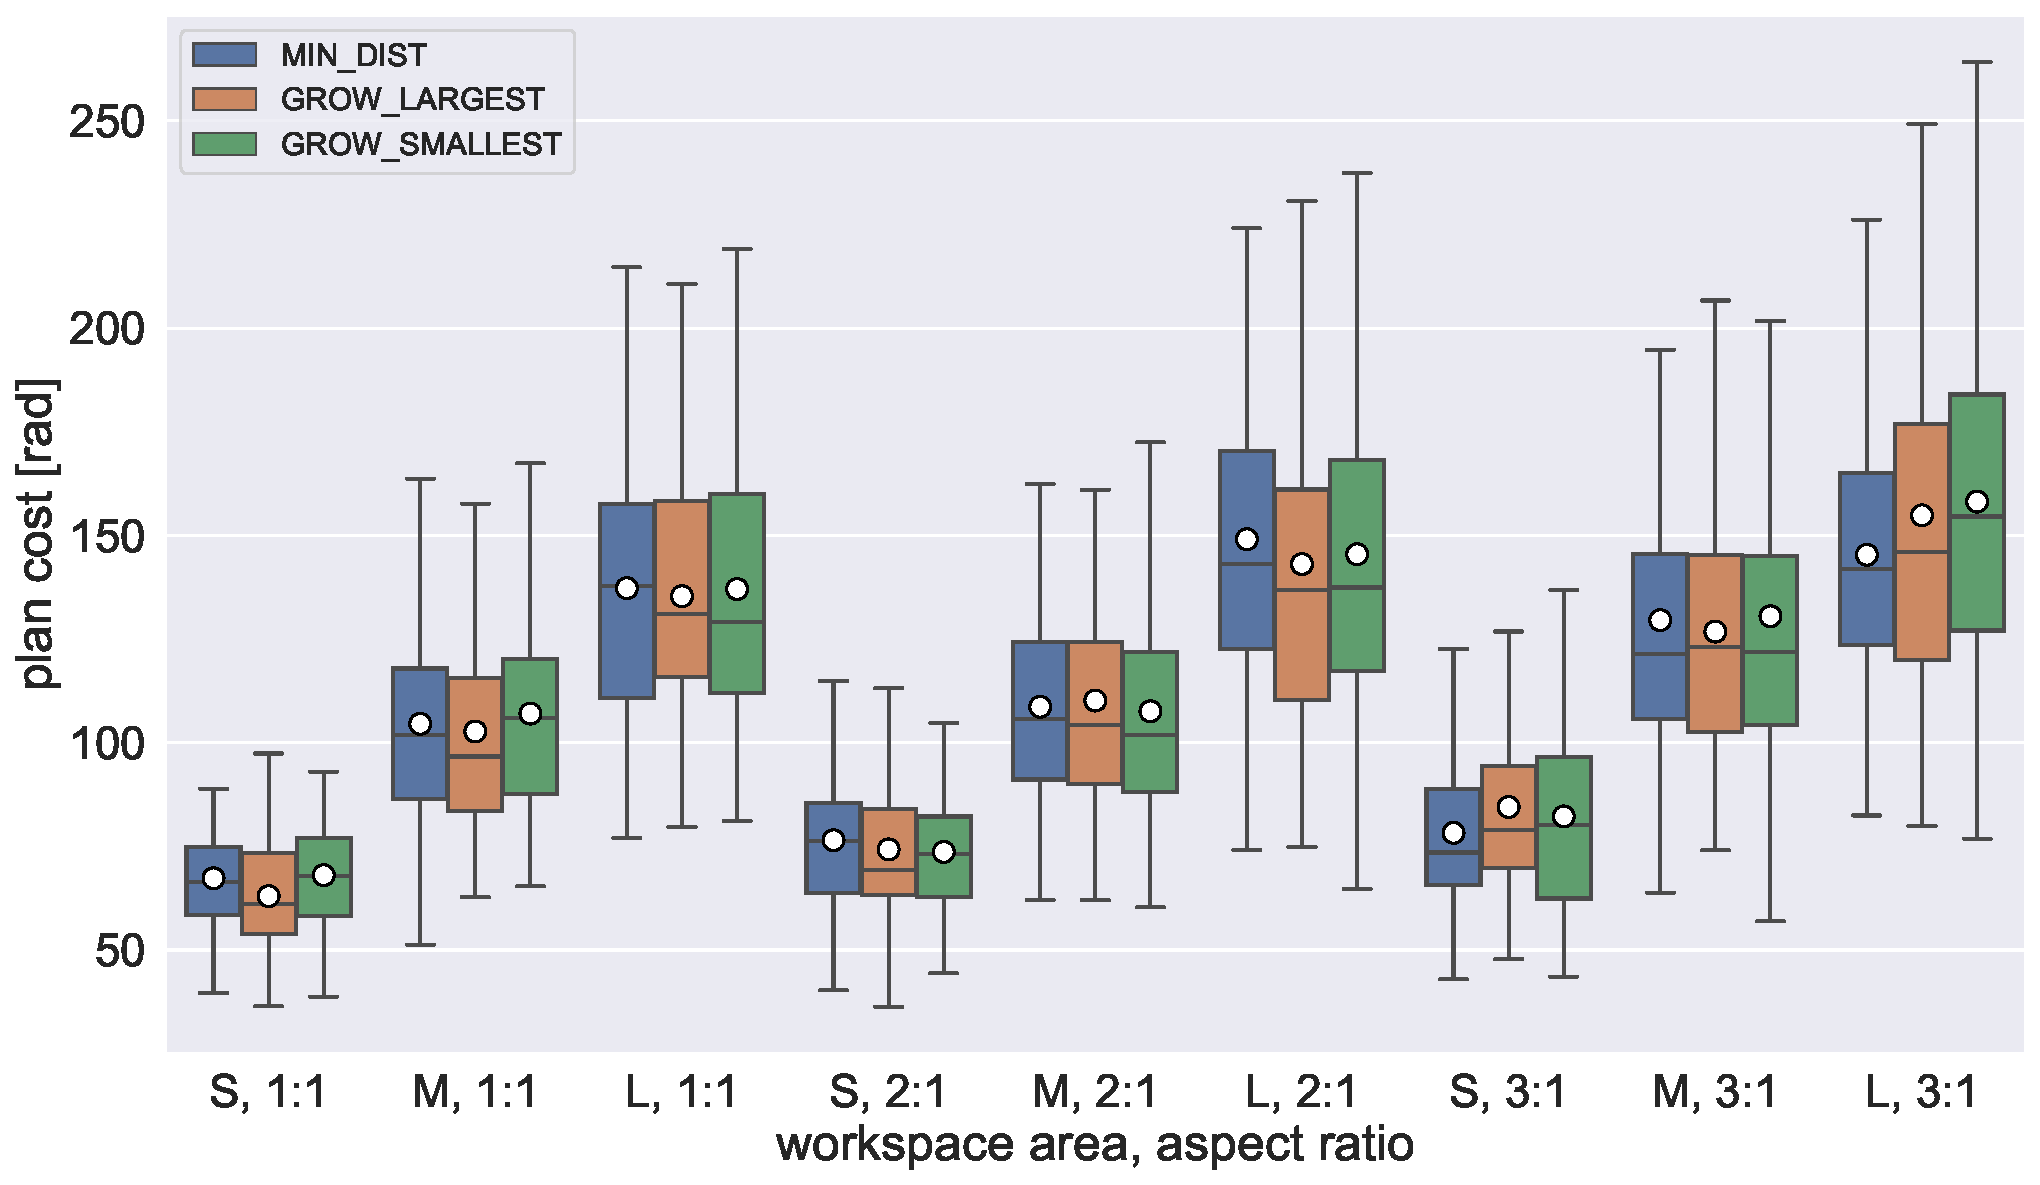
\includegraphics[width=0.9\textwidth]{figures/plots/AFBS_cost.pdf}
	\caption[]{}
	\label{fig:AFBS_cost}
\end{figure}



